\section{Sturm-Liouville Theory}\label{sec:slmain}

Sturm-Liouville Theory is the theory of second-order boundary value eigenproblems of the form
\begin{equation}
	-\left(p(x)y'\right)' + q(x)y = \lambda r(x)y, \quad y(0)=y(1)=0.
\end{equation}

\subsection{Motivation}

Two ideas motivate Sturm-Liouville theory.

\begin{enumerate}
	\item \textbf{Eigenvalues of symmetric matrices.}
	
	The eigenvalues and eigenvectors of a symmetric matrix may be represented as follows:
	\begin{equation}\label{eq:sleigs}
		A\xib_n = \lambda_n\xib_n, \quad A^T = A.
	\end{equation}
	The following properties are equivalent to the condition of a matrix being symmetric:
	\begin{itemize}
		\item $\bm{u} \cdot A\bm{v} = \bm{v} \cdot A\bm{u}$, $\forall \bm{u},\bm{v}$,
		\item $\xib_m\cdot\xib_n = 0$ for $m \neq n$.
	\end{itemize}
	We can see that the second property follows from the first by taking the dot product of $\xib_m$ and $\xib_n$ (for $m\neq n$) with \Cref{eq:sleigs},
	\begin{align*}
		\xib_m\cdot A\xib_n &= \xib_m\cdot(\lambda_n\xib_n) = \lambda_n \xib_m\cdot\xib_n \\
		\xib_n\cdot A\xib_m &= \lambda_m \xib_n\cdot\xib_m.
	\end{align*}
	Taking the difference of these two equations yields
	\[
	\xib_m\cdot A\xib_n - \xib_n\cdot A\xib_m = (\lambda_n - \lambda_m)\xib_n\cdot\xib_m = 0,
	\]
	since $\xib_m\cdot A\xib_n = \xib_n\cdot A\xib_m$ from the first property. Therefore if $\lambda_m \neq \lambda_n$, we can conclude that $\xib_m\cdot\xib_n = 0$ for $m \neq n$.
	
	\item \textbf{Fourier series with eigenfunctions} $X_n(x) = \sin\left(\frac{n\pi x}{L}\right)$.
	
	From the definition of eigenvalues and eigenfunctions, we know that\footnote{In this equation, the $L$ in $LX_n$ represents the linear map defined in \Cref{eg:linearmap}, while $L$ in $X_n(L)$ is a scalar related to the period of the function. Generally, common sense should be enough to determine which is which.}
	\[
	LX_n = X_n'' = \lambda_n X_n, \quad X_n(0) = X_n(L) = 0.
	\]
	We know that these functions $X_n$ are orthogonal (where orthogonality was defined in \Cref{eq:innerprod}), therefore $(X_m, X_n) = 0$ for $m \neq n$. From the definition of orthogonality, we can see that
	\begin{align*}
		(X_m, LX_n) &= \lambda_n (X_m, X_n) \\
		(X_n, LX_m) &= \lambda_m (X_n, X_m).
	\end{align*}
	Therefore
	\begin{align*}
		(\lambda_n - \lambda_m)(X_m, X_n) &= (X_m, LX_n) - (X_n, LX_m) \\
		&= \int_0^L X_mX_n'' - X_m''X_n\,dx \\
		&= \cancelto{0}{\left[X_mX_n'\right]_0^L} - \cancel{\int_0^LX_m'X_n' \,dx} - \cancelto{0}{\left[X_m'X_n\right]_0^L} + \cancel{\int_0^L X_m'X_n' \,dx} \\
		&= 0
	\end{align*}
	Since $(\lambda_n - \lambda_m)(X_m, X_n) = 0$, we find that $(X_m,X_n) = 0$ when $\lambda_m \neq \lambda_n$ and $m \neq n$.
	
	Therefore, we have established orthogonality of the functions $X_n(x) = \sin\left(\frac{n\pi x}{L}\right)$ without using trigonometry: the only fact we needed was that these sine functions satisfy the eigenvalue problem.
\end{enumerate}

Thus, we have learned that if $L = \frac{d^2}{dx^2}$, then
\begin{equation}
	(u, Lv) - (v, Lu) = 0, \quad \forall u,v,
\end{equation}
where
\[
(u,v) = \int_0^1 u(x)v^*(x) \,dx
\]
(compare this to \Cref{eq:innerprodcomplex}.) This is called \textbf{Lagrange's Identity}.

Operators that satisfy this property are equivalent to symmetric matrices and are called self-adjoint operators. Thus, essentially everything we know about symmetric matrices (e.g. orthogonal eigenvectors, real eigenvalues, etc.) will hold when working with these operators.

\subsection{Sturm-Liouville Eigenvalue Problems}

\begin{definition}
	The eigenvalue ODE equation
	\begin{equation}\label{eq:sturmliou}
		Ly = -\left(p(x)y'\right)' + q(x)y = \lambda r(x)y, \quad 0 \leq x \leq 1,
	\end{equation}
	subject to the boundary conditions
	\begin{equation}\label{eq:sturmliouconds}
		\begin{alignedat}{1}
			a_1y(0) + a_2y'(0) &= 0 \\
			b_1y(1) + b_2y'(1) &= 0.
		\end{alignedat}
	\end{equation}
	defines a (regular) \textbf{Sturm-Liouville boundary problem}, where the functions $p$, $q$, $r$, and $p'$ are continuous and $p$ and $r$ are strictly positive.
\end{definition}

We will make use of Lagrange's Identity which was stated in the previous section, i.e. that
\[
(u, Lv) = (v, Lu).
\]
We can prove this without too much trouble for the problems of the form in \Cref{eq:sturmliou}.

\begin{proof}
	\begin{align*}
		(u, Lv) &= \int_0^1 u\left(-(pv^{*\prime})' + qv^*\right) \,dx \\
		&= \left[-puv^{*\prime}\right]_0^1 + \int_0^1 pu'v^{*\prime} + quv \,dx \\
		&= \left[-puv^{*\prime}\right]_0^1 + \left[pu'v^*\right]_0^1 + \int_0^1 (-(pu')' + qu)v^* \,dx \\
		&= \left[pu'v^*-puv^{*\prime}\right]_0^1 + \int_0^1 Luv^* \,dx \\
		&= p(1)\left(u'(1)v^*(1) - u(1)v^{*\prime}(1)\right) - p(0)\left(u'(0)v^*(0) - u(0)v^{*\prime}(0)\right) + (Lu, v).
	\end{align*}
	But from \Cref{eq:sturmliouconds},
	\[
	u'(1) = -\frac{a_2}{a_1}u(1) \quad\text{and}\quad v^{*\prime}(1) = -\frac{a_2}{a_1}v^*(1)
	\]
	therefore
	\begin{align*}
		u'(1)v^*(1) - u(1)v^{*\prime}(1) &= 0 \\
		u'(0)v^*(0) - u(0)v^{*\prime}(0) &= 0
	\end{align*}
	and so we have proved that
	\[
	(u, Lv) = (Lu, v) = (v, Lu).
	\]
\end{proof}

Properties:
\begin{enumerate}
	\item The eigenvalues are real, $\lambda_n \in \R$.
	\item The eigenfunctions are orthogonal:
	\[
	\langle \phi_m, \phi_n \rangle = \int_0^1 \phi_m(x)\phi_n^*(x)r(x) \,dx = (\phi_m, r\phi_n) = 0 \quad \text{if } \lambda_m \neq \lambda_n.
	\]
\end{enumerate}

\begin{proof}\leavevmode
	\begin{enumerate}
		\item We apply Lagrange's Identity to $u = \phi_n$ and $u = \phi_n$, noting that we have $L \phi_n = \lambda_n r\phi_n$ since we are dealing with problems of the form in \Cref{eq:sturmliou}. Then
		\begin{align*}
			&(L\phi_n, \phi_n) = (\phi_n, L\phi_n) \\
			\implies &(\lambda_n r\phi_n, \phi_n) = (\phi_n, \lambda_n r\phi_n) \\
			\implies &\lambda_n(r\phi_n, \phi_n) = \lambda_n^*(\phi_n, r\phi_n) \\
			\implies &(\lambda_n - \lambda_n^*) \underbrace{\int_0^1 r |\phi_n|^2 \,dx}_{\neq 0} = 0 \\
			\implies &\lambda_n = \lambda_n^* \text{ i.e. } \lambda_n \in \R. 
			\intertext{\item We apply Lagrange's identity to $u = \phi_n$, $v = \phi_m$. Then}
			&(L\phi_n, \phi_m) = (\phi_n, L\phi_m) \\
			\implies &(\lambda_n r\phi_n, \phi_m) = (\phi_n, \lambda_m r\phi_m) \\
			\implies &(\lambda_n - \lambda_m)(r\phi_n, \phi_m) = 0 \tag{$\lambda_n = \lambda_n^*$} \\
			\implies &(r\phi_n, \phi_m) = 0 \text{ for } \lambda_n \neq \lambda_m.
		\end{align*}
		Therefore $\langle \phi_m, \phi_n \rangle = 0$ also.
	\end{enumerate}
\end{proof}

\begin{remark}
	As the eigenvalues are real, so too are the eigenfunctions.
\end{remark}

\begin{theorem}
	The eigenvalues form an ordered sequence
	\[
	\lambda_1 < \lambda_2 < \cdots < \lambda_n \to \infty,
	\]
	and there is a unique eigenfunction for each $\lambda_n$.
\end{theorem}

\begin{proof}
	Me providing a proof that everyone can use is basically socialism. Pull yourself up by your bootstraps and create a proof yourself.
\end{proof}

\begin{eg}\label{eg:sl1}
	We solve the following Sturm-Liouville problem:
	\[
	-y'' = \lambda y, \quad\text{with}\quad y(0)=0,\,\, y(1) + y'(1) = 0.
	\]
	As is typical for solving this sort of problem, we split it into three cases depending on whether $\lambda$ is positive, negative, or zero:
	\begin{itemize}
		\item Case 1: $\lambda = \mu^2 > 0$. Then the solution is
		\[
		y(x) = A\cos(\mu x) + B\sin(\mu x)
		\]
		Applying the boundary conditions,
		\begin{align*}
			y(0) &= A = 0 \\
			y(1) + y'(1) &= B\sin\mu + \mu B\cos\mu = 0 \text{ where } \tan\mu = -\mu.
		\end{align*}
		This has infinitely many solutions (graph the functions to see this), therefore we have eigenvalues of the form $\lambda_n = \mu_n^2$ and eigenfunctions $Y_n(x) = \sin(\mu_n x) = \sin(\sqrt{\lambda_n}x)$ for $n \in \mathbb{N}$, where $\mu_n$ is the $n$th solution of the equation $\tan\mu = -\mu$.
		
		\item Case 2: $\lambda = 0$. The solution is
		\[
		y(x) = Ax + B,
		\]
		and applying the boundary conditions yields
		\begin{align*}
			y(0) &= B = 0 \\
			y(1) + y'(1) &= 2A = 0,
		\end{align*}
		hence we only have trivial solutions in this case.
		
		\item Case 3: $\lambda = -\mu^2 < 0$. The solution is
		\[
		y(x) = A\cosh(\mu x) + B\sinh(\mu x),
		\]
		and similar to Case 1, applying the boundary conditions yields the condition $\tanh\mu = -\mu$, which has no solutions except the trivial $\mu = 0$.
	\end{itemize}
	Therefore, the only solutions to this problem are those from Case 1.
\end{eg}

\subsubsection{Normalisation of Eigenfunctions}\label{sec:normaleigenfuncs}

In the previous example, we found that the eigenfunctions were such that
\[
\phi_n = k_n \sin(\sqrt{\lambda_n}x).
\]

What we can do is impose the condition $\langle \phi_n, \phi_n \rangle = 1$ to make these functions orthonormal as well as orthogonal. We can calculate the values of $k_n$ as follows:
\begin{align*}
	1 &= k_n^2 \int_0^1 \sin^2(\sqrt{\lambda_n} x) \,dx = \frac{k_n^2}{2} \int_0^1 1 - \cos(2\sqrt{\lambda_n}x) \,dx \\
	&= \frac{k_n^2}{2} \left(1 - \frac{\sin(2\sqrt{\lambda_n})}{2\sqrt{\lambda_n}}\right) = \frac{k_n^2}{2} \left(1 - \frac{2\sin\sqrt{\lambda_n}\cos\sqrt{\lambda_n}}{2\sqrt{\lambda_n}}\right) \\
	\intertext{From \Cref{eg:sl1}, we found that $\sin\mu + \mu\cos\mu = 0 \implies \frac{1}{\sqrt{\lambda_n}}\sin\sqrt{\lambda_n} = -\cos\sqrt{\lambda_n}$. Making this substitition yields}
	&= \frac{k_n^2}{2} (1 + \cos^2\sqrt{\lambda_n}) \\
	k_n &= \left(\frac{2}{1 + \cos^2\sqrt{\lambda_n}}\right)^{\frac12}.
\end{align*}

\subsection{Further Results on Sturm-Liouville Problems}

Eigenfunctions of Sturm-Liouville provide a complete basis in which to expand functions. We use this to solve some inhomogeneous boundary-value problems and some PDEs.
Sturm-Liouville problems are eigenvalue problems where 
\begin{equation}\label{eq6.2.1}
	L[\phi_n] = \lambda_n r(x) \phi_n
\end{equation}
\[
L[u] = -(pu')' + qu
\]

Note that $L[u]$ in the above equation is called the Sturm-Liouville Operator.

If we look at the boundary conditions for \Cref{eq6.2.1}, they must satisfy the Lagrange identity, i.e., if we have two functions $u, v$ which satisfy the same boundary conditions as $\phi_n$, then
\[
	(Lu, v) = (u, Lv).
\]
The other inner product is also useful:
\[
	\langle \phi_m, \phi_n\rangle = (\phi_m, r\phi_n) = \int_0^1 \phi_m(x) \phi_n(x) r(x) \,dx = \delta_{mn} = \begin{cases} 0 & \text{if } m \neq n \\ 1 & \text{if } m = n \end{cases}
\]

\subsubsection{Expanding Functions}\label{sec:slexpand}

We now want to expand any function in the basis made up of the eigenfunctions $\phi_n$:
\[
f(x) = \sum_{n=1}^{\infty}c_n \phi_n(x)
\]
So if the expansion holds, we can find $c_n$ by projecting $f$ on $\phi_m$
\begin{align*}
	\langle f, \phi_m\rangle &= \sum_{n=1}^{\infty} c_n \underbrace{\langle \phi_n, \phi_m\rangle}_{=\delta_{mn}} = c_m
\end{align*}
The formula
\[
c_m = \langle f, \phi_n\rangle
\]
is essentially a generalisation of the Euler-Fourier formulas, which gave the expansion for functions $\phi_n$ in terms of cosines and sines.

\begin{eg}\label{eg:slexpand}
	Expand the function $f(x) = x$ in the interval $0<x<1$ using the orthonormal set from \Cref{eg:sl1}:
	\[
		f(x) = x = \sum_{n=1}^{\infty} c_n \phi_n \quad\text{with}\quad \phi_n = k_n \sin(\sqrt{\lambda_n} x).
	\]
	Using orthonormality, the unknown coefficients are fixed by
	\begin{align*}
		c_n &= k_n \int_0^1 x \sin(\sqrt{\lambda_n} x) \,dx \\
		&= k_n \left( \left[-\frac{x}{\sqrt{\lambda_n}}\cos(\sqrt{\lambda_n} x)\right]_0^1 + \int_0^1 \frac{1}{\sqrt{\lambda_n}} \cos(\sqrt{\lambda_n} x) \,dx \right) \\
		&= k_n\left( -\frac{1}{\sqrt{\lambda_n}}\cos\sqrt{\lambda_n} + \left[\frac{1}{\lambda_n} \sin(\sqrt{\lambda_n} x)\right]_0^1 \right) \\
		&= k_n\left( -\frac{1}{\sqrt{\lambda_n}}\cos\sqrt{\lambda_n} + \frac{1}{\lambda_n} \sin\sqrt{\lambda_n} \right)
		\intertext{Using the relation $\cos\sqrt{\lambda_n}= -\frac{1}{\sqrt{\lambda_n}}\sin\sqrt{\lambda_n}$ like in \Cref{sec:normaleigenfuncs}}
		&= k_n\left( \frac{1}{\lambda_n}\sin\sqrt{\lambda_n} + \frac{1}{\lambda_n} \sin\sqrt{\lambda_n} \right) \\
		&= k_n \frac{2\sin\sqrt{\lambda_n}}{\lambda_n} \\
		&= \frac{2\sqrt{2} \sin\sqrt{\lambda_n}}{\lambda_n (1 + \cos^2\sqrt{\lambda_n})^{1/2}},
	\end{align*}
	where in the last line we use the value for $k_n$ calculated in \Cref{sec:normaleigenfuncs}.
	
	Therefore the series is given by
	\begin{align*}
		f(x) &= \sum_{n=1}^{\infty} c_n k_n \sin(\sqrt{\lambda_n}x) \\
		&= \sum_{n=1}^{\infty} \frac{2\sqrt{2} \sin(\sqrt{\lambda_n})}{\lambda_n (1 + \cos^2\sqrt{\lambda_n})^{1/2}} \cdot \frac{\sqrt{2}}{(1 + \cos^2\sqrt{\lambda_n})^{1/2}} \sin(\sqrt{\lambda_n}x) \\
		&= 4\sum_{n=1}^{\infty} \frac{\sin\sqrt{\lambda_n}}{\lambda_n (1 + \cos^2\sqrt{\lambda_n})} \sin(\sqrt{\lambda_n}x).
	\end{align*}
\end{eg}

\subsubsection{Convergence Theorem}

We wish to consider the convergence of the series
\[
\sum_{n=1}^{\infty} c_n \phi_n(x) \quad\text{with}\quad c_n = \langle f, \phi_n\rangle
\]
\begin{theorem}
	Assume $f$ and $f'$ are piecewise continuous. Then $\sum_{n=1}^{\infty} c_n \phi_n(x)$ converges:
	\begin{itemize}
		\item to $f(x)$ where $f$ is continuous,
		\item to $\frac{f(x_+)+f(x_-)}{2}$ (i.e. the midpoint of the left and right endpoints) elsewhere.
	\end{itemize}
\end{theorem}

We can also state an analogous formula for Parseval's Identity:
\begin{equation}
	\langle f,f\rangle = \int_0^1 f^2(x)r(x)dx = \sum_{n=1}^{\infty} c_n^2.
\end{equation}

\begin{proof}
	\[
	\langle f,f\rangle = \left\langle \sum_{n=1}^{\infty} c_n \phi_n, \sum_{m=1}^{\infty} c_m \phi_m\right\rangle = \sum_{n=1}^{\infty} \sum_{m=1}^{\infty} c_n c_m \underbrace{\langle \phi_n, \phi_m\rangle}_{=\delta_{mn}} = \sum_{n=1}^{\infty} c_n^2.
	\]
\end{proof}

Compare these with the Fourier convergence theorem (\Cref{thrm:fourierconv}) and Parseval's theorem (\Cref{thrm:parseval}).


\subsubsection{Non-homogenous Boundary Value Problems}

The non-homogeneous Sturm-Liouville boundary value problem is given by
\begin{equation}\label{eq6.2.2}
	L[y] = \mu r(x) y + f(x),
\end{equation}
with Sturm-Liouville boundary conditions.

First, we solve the corresponding homogeneous Sturm-Liouville boundary problem
\[
	L[y] = \lambda r(x)y
\]
subject to the same boundary conditions. This eigenvalue problem determines an orthonormal set of functions $\phi_n(x)$ satisfying
\[
	L[\phi_n] = \lambda_n r(x) \phi_n(x).
\]

We expand the solution to the non-homogeneous ODE into this basis
\[
	y(x) = \sum_{n=1}^{\infty} b_n \phi_n(x).
\]
Substitution into the non-homogeneous ODE from \Cref{eq6.2.2} yields
\begin{align*}
	\sum_{n=1}^{\infty} b_n L \phi_n = r(x) \sum_{n=1}^{\infty} b_n \lambda_n \phi_n(x) &= r(x) \sum_{n=1}^{\infty} \mu b_n \phi_n(x) + f(x) \\
	\implies \sum_{n=1}^{\infty} b_n (\lambda_n - \mu) \phi_n(x) &= \frac{f(x)}{r(x)}.
\end{align*}
Expanding the RHS in the same basis, as in \Cref{sec:slexpand}:
\[
	\frac{f(x)}{r(x)} = \sum_{n=1}^{\infty} c_n \phi_n(x) \quad\text{with}\quad c_n = \left\langle \frac{f}{r}, \phi_n \right\rangle = \int_0^1 r(x) \frac{f(x)}{r(x)} \phi_n(x) \,dx = (f, \phi_n),
\]
then the non-homogeneous ODE yields
\[
	\sum_{n=1}^{\infty} [b_n(\lambda_n - \mu) - c_n] \phi_n(x) = 0.
\]
Since $\phi_n(x)$ are orthogonal, each coefficient must vanish:
\begin{itemize}
	\item If $\mu \neq \lambda_n$, $n = 1, 2, \ldots$, then each solution is unique,
	\[
		b_n = \frac{c_n}{\lambda_n - \mu}.
	\]
	\item If there exists $m$ such that $\mu = \lambda_m$, we have the condition
	\[
		b_m \cdot 0 - c_m = 0.
	\]
	If $c_m = \langle \frac{f(x)}{r(x)}, \phi_m(x)\rangle = 0$, this equation is satisfied and there are infinitely many solutions as $b_m$ is undetermined. If $c_m \neq 0$, there is no solution.
\end{itemize}

\begin{eg}
	Solve
	\[
		y'' + 2y = -x, \quad y(0) = y(1) + y'(1) = 0.
	\]
	Using the methods we already know for solving such IVPs (method of undetermined coefficients), we can find the solution to be
	\[
		y(x) = \frac{\sin(\sqrt{2}x)}{\sin\sqrt{2} + \sqrt{2}\cos\sqrt{2}} - \frac{x}{2},
	\]
	but it still serves as a good example to illustrate the Sturm-Liouville method we just discussed. Here, we solve
	\[
		-y'' = 2y + x,
	\]
	using the auxiliary (homogeneous) Sturm-Liouville boundary value problem
	\[
		-y'' = \lambda y, \quad\text{with}\quad y(0) = y(1) + y'(1) = 0.
	\]
	From \Cref{eg:sl1} and \Cref{sec:normaleigenfuncs}, the solution to this BVP are given by orthonormal functions $\phi_n(x) = k_n \sin(\sqrt{\lambda_n}x)$, with
	\[
		\sin\sqrt{\lambda_n} + \sqrt{\lambda_n}\cos\sqrt{\lambda_n} = 0 \quad\text{and}\quad k_n = \left(\frac{2}{1 + \cos^2\sqrt{\lambda_n}}\right)^{\frac12}.
	\]
	Since the set $\{\phi_n(x)\}$ provides a complete basis of functions, we can expand the solution as
	\[
		y(x) = \sum_{n=1}^{\infty} b_n \phi_n(x),
	\]
	with unknown coefficients $\{b_n\}$. Furthermore, from \Cref{eg:slexpand} we can expand the inhomogeneous function as
	\[
		x = \sum_{n=1}^{\infty} c_n \phi_n(x), \quad\text{where}\quad c_n = \frac{2\sqrt{2} \sin\sqrt{\lambda_n}}{\lambda_n (1 + \cos^2\sqrt{\lambda_n})^{1/2}}.
	\]
	Then
	\[
		y(x) = \sum_{n=1}^{\infty} b_n \phi_n(x) \implies y'' = \sum_{n=1}^{\infty} b_n \phi''_n(x) = \sum_{n=1}^{\infty} b_n\lambda_n\phi_n(x).
	\]
	Plugging into the non-homogeneous ODE:
	\[
		\sum_{n=1}^{\infty} b_n(-\lambda_n + 2)\phi_n(x) = -\sum_{n=1}^{\infty} c_n \phi_n(x).
	\]
	Since $\phi_n(x)$ are orthogonal, we can conclude
	\[
		b_n = \frac{c_n}{\lambda_n - 2}.
	\]
	Note that the solution is unique since $\lambda_n \neq 2$ (because $\sin\sqrt{2} + \sqrt{2}\cos\sqrt{2} \neq 0$).
\end{eg}


\subsubsection{Non-homogeneous PDEs}

\begin{eg}
	As an example, we consider the generalised heat equation:
	\[
		r(x) \p_t u(x,t) = \p_x\left(p(x) \p_x u(x,t)\right) - q(x) u(x,t) + f(x,t),
	\]
	where $\p_x\left(p(x) \p_x u\right) - q(x) u = L[u]$ and the boundary conditions are
	\begin{align*}
		\p_x u(0,t) - h_1 u(0,t) &= 0 \\
		\p_x u(1,t) - h_2 u(1,t) &= 0 \\
		u(x,0) &= f(x).
	\end{align*}
	
	We will follow a similar strategy to the one discussed for ODEs. First, consider the Sturm-Liouville boundary problem associated with the homogeneous PDE
	\[
		r(x) \p_t u(x,t) = \p_x\left(p(x) \p_x u(x,t)\right) - q(x) u(x,t).
	\]
	The separation of variables $u(x,t) = X(x)T(t)$ yields
	\[
		rXT' = [PX'T]' - qXT \implies \frac{T'}{T} = \frac{1}{rX}[pX']' - \frac{q}{e} = -\lambda,
	\]
	thus
	\begin{align*}
		T' &= -\lambda T \\
		-(pX')' + qX &= \lambda rX
	\end{align*}
	satisfying $X'(0) - h_1X(0) = X'(1) + h_2X(1) = 0$.
	
	Assume the Sturm-Liouville boundary problem is solved - that is, there exist a set of eigenvalues $\{\lambda_n\}$ associated with orthonormal eigenfunctions $\{\phi_n(x)\}$. We now look for a solution to the non-homogeneous PDE by expanding in this basis
	\[
		u(x,t) = \sum_{n=1}^{\infty} b_n(t) \phi_n(x).
	\]
	We can expand $f(x,t)$ in the same basis:
	\[
		\frac{f(x,t)}{r(x)} = \sum_{n=1}^{\infty} \gamma_n(t) \phi_n(x), \quad\text{with}\quad \gamma_n(t) = \left\langle \frac{f(x,t)}{r(x)}, \phi(x) \right\rangle = \int_0^1 r(x) \frac{f(x,t)}{r(x)} \phi_n(x) \,dx.
	\]
	When we substitute this into the non-homogeneous PDE, we get
	\[
		r(x) \sum_{n=1}^{\infty} \dot{b}_n(t) \phi_n(x) = \sum_{n=1}^{\infty} b_n(t) \left([p(x)\phi'_n(x)]' - q(x)\phi_n(x)\right) + f(x,t).
	\]
	Since $\phi_n(x)$ satisfies the Sturm-Liouville boundary problem, it satisfied
	\[
		[p(x)\phi'_n(x)]' - q(x)\phi_n(x) = \lambda_n r(x) \phi_n(x),
	\]
	so our non-homogeneous PDE yields
	\begin{align*}
		r(x) \sum_{n=1}^{\infty} \dot{b}_n(t) \phi_n(x) &= -r(x)\sum_{n=1}^{\infty} b_n(t) \lambda_n \phi_n(x) + f(x,t) \\
		\implies \sum_{n=1}^{\infty} \dot{b}_n(t) \phi_n(x) &= \sum_{n=1}^{\infty} b_n(t) \lambda_n \phi_n(x) + \sum_{n=1}^{\infty} \gamma_n(t) \phi_n(x).
	\end{align*}
	Thus
	\[
		\sum_{n=1}^{\infty} \left[\dot{b}_n(t) + \lambda_n b_n(t) - \gamma_n(t)\right] \phi_n(x) = 0,
	\]
	and using the orthogonality of the set $\{\phi_n(x)\}$, we can conclude
	\[
		\dot{b}_n(t) + \lambda_n b_n(t) = \gamma_n(t), \quad n = 1, 2, 3, \ldots
	\]
	This is an infinite countable set of linear first-order ODEs, which can each be solved with the integrating factor $\exp(\lambda_n t)$:
	\begin{align}
		\frac{d}{dt}(e^{\lambda_n t}b_n) &= e^{\lambda_n t}\gamma_n \implies e^{\lambda_n t}b_n = \int_0^t e^{\lambda_n s}\gamma(s) \,ds + \alpha_n \nonumber \\
		\label{eq:slpdesbn}
		\implies b_n(t) &= e^{\lambda_n t} \int_0^t e^{\lambda_n s}\gamma(s) \,ds + e^{-\lambda_n t}\alpha_n, \quad\text{with}\quad \alpha_n = b_n(0).
	\end{align}
	The initial values $b_n(0)$ are determined from
	\begin{align*}
		u(x,0) &= \sum_{n=1}^{\infty} b_n(0)\phi_n(x) = f(x) \\
		\implies b_n(x) &= \langle f, \phi_n\rangle = \int_0^1 r(x)f(x)\phi_n(x)\,dx = \alpha_n.
	\end{align*}
	In conclusion, the general solution to the non-homogeneous PDE boundary problem is
	\[
		u(x,t) = \sum_{n=1}^{\infty} b_n(t)\phi_n(x),
	\]
	where the set $\{b_n(t)\}$ is given as above in \Cref{eq:slpdesbn} and the set $\{\phi_n(x)\}$ solved the auxiliary Sturm-Liouville boundary problem.
\end{eg}

Solving these types of problems in practice is illustrated in Examples 1 and 2 of Section 11.3 of Boyce.

In summary, the strategy for solving non-homogeneous PDEs is:
\begin{itemize}
	\item Find the eigenvalues $\lambda_n$ and normalised eigenfunctions $\phi_n$ of the corresponding homogeneous problem.
	\item Calculate coefficients $\gamma_n(t)$ and $\alpha_n$.
	\item Evaluate the integrals for $b_n(t)$.
	\item Sum the infinite series of $b_n(t) \phi_n(x)$ terms.
\end{itemize}


\subsubsection{Transforming ODEs into Sturm-Liouville Form}

In this section, we show that any second-order ODE of the form
\begin{equation}\label{eq:sltransform}
	a_2(x)y'' + a_1(x)y' + a_0(x)y = \lambda f(x)y
\end{equation}
can be transformed into the Sturm-Liouville form from \Cref{eq:sturmliou}
\begin{equation}\label{eq:sltransform2}
	-\left(p(x)y'\right)' + q(x)y = \lambda r(x)y, \quad 0 \leq x \leq 1.
\end{equation}

For this transformation, what we essentially seek is an integrating factor $\mu(x)$ to do this transformation. To find this factor, we being with \Cref{eq:sltransform}, divide by $a_2(x)$ and multiply by $\mu(x)$:
\begin{align*}
	a_2(x)y'' + a_1(x)y' + a_0(x)y &= \lambda f(x)y \\
	y'' + \frac{a_1(x)}{a_2(x)}y' + \frac{a_0(x)}{a_2(x)}y &= \frac{f(x)}{a_2(x)}\lambda y \\
	\mu(x)y'' + \mu(x)\frac{a_1(x)}{a_2(x)}y' + \mu(x)\frac{a_0(x)}{a_2(x)}y &= \mu(x)\frac{f(x)}{a_2(x)}\lambda y.
\end{align*}

In order for the terms $\mu(x)y'' + \mu(x)\frac{a_1(x)}{a_2(x)}y'$ to be written as $-(p(x)y')'$, we require
\[
\mu'(x) = \mu(x)\frac{a_1(x)}{a_2(x)}.
\]
This is solved as a separable first-order differential equation:
\begin{align*}
	\mu'(x) = \frac{d\mu}{dx} &= \mu(x)\frac{a_1(x)}{a_2(x)} \\
	\frac{d\mu}{\mu} &= \frac{a_1(x)}{a_2(x)} dx \\ 
	\ln\mu &= \int_{x_0}^x \frac{a_1(s)}{a_2(s)} \,ds \\
	\mu(x) &= \exp\left(\int_{x_0}^x \frac{a_1(s)}{a_2(s)} \,ds\right).
\end{align*}
In other words, multiplying through by this factor $\mu(x)$ and dividing by $a_2(x)$ converts the ODE into the desired form.\footnote{Though it might be required to put multiply the entire equation by $(-1)$ if we want $-(p(x)y')'$ instead of $(p(x)y')'$.}

So, in summary, any ODE of the form in \Cref{eq:sltransform} can be transformed into the Sturm-Liouville form in \Cref{eq:sltransform2}, where
\begin{align*}
	p(x) &= -\exp\left(\int_{x_0}^x \frac{a_1(s)}{a_2(s)} \,ds\right) \\
	q(x) &= -p(x)\frac{a_0(x)}{a_2(x)} \\
	r(x) &= -p(x)\frac{f(x)}{a_2(x)}.
\end{align*}

\begin{eg}
	Consider the ODE
	\[
	xy'' + (1-x\tan{x})y' + x^2y = \lambda y.
	\]
	We find the integrating factor $\mu(x)$ as follows
	\begin{align*}
		\mu(x) &= \exp\left(\int \frac{a_1(x)}{a_2(x)} \,dx\right) = \exp\left(\int \frac{1+x\tan{x}}{x} \,dx\right) \\
		&= \exp\left(\int \frac{1}{x} + \tan{x} \,dx\right) = \exp\left(\ln{x} + \ln|\cos{x}|\right) \\
		&= x\cos{x},
	\end{align*}
	where we can write $|\cos(x)| = \cos(x)$ since cosine is positive on the interval $[0,1]$. Next, multiplying by $\mu(x)/a_2(x) = \cos(x)$:
	\begin{align*}
		x\cos(x)y'' + (1-x\tan(x))\cos(x)y' + x^2\cos(x)y &= \lambda \cos(x)y \\
		x\cos(x)y'' + (\cos(x)-x\sin(x))y' + x^2\cos(x)y &= \lambda \cos(x)y \\
		\left(x\cos(x)y'\right)' + x^2\cos(x)y &= \lambda \cos(x)y,
	\end{align*}
	which is in SL form (or, if we wish to be precise, we can multiply by $(-1)$ to reach the form of \Cref{eq:sltransform2}).
\end{eg}

\subsection{Singular Sturm-Liouville Problems and the Bessel Equation}\label{sec:singularsl}

Recall that the general Sturm-Liouville Problems are given by
\[
	L[y] = -\left(p(x)y'\right)' + q(x)y = \lambda r(x) y \qquad 0 \leq x \leq 1.
\]
where it is assumed that $p$ is differentiable, $q$ and $r$ are continuous, and $p(x)>0$, $r(x)>0$ at all points in the closed interval $[0,1]$.

But for some problems of physical interest these conditions are satisfied only for the open interval $(0,1)$. Sturm–Liouville problems for which the conditions on $p$, $q$ and $r$ are satisfied on $0 < x < 1$ but are not satisfied at $x = 0$ and/or $x = 1$ are called \textbf{singular}.


\begin{eg}[Bessel's equation of order $m$]\label{eg:bessel}
	\[
	-\left(xy'\right)' + \frac{m^2}{x}y = \lambda xy, \quad\text{with}\quad y(x) \text{ bounded as } x \rightarrow 0, \,\, y(1) = 0
	\]
	In other words, we have
	\begin{align*}
		p(x) = x, \quad q(x) = \frac{m^2}{x}, \quad r(x) = x.
	\end{align*}
	The problem can also be written as 
	\[
	y'' + \frac{1}{x} y' + \left(\lambda - \frac{m^2}{x^2}\right)y = 0.
	\]
	Let $t= \sqrt{\lambda} x$. Then
	\begin{align}
		\lambda\frac{d^2y}{dt^2} + \frac{\lambda}{t} \frac{dy}{dt} + \lambda\left(1- \frac{m^2}{t^2}\right)y &= 0 \nonumber \\
		\label{eq:bessel}\implies \frac{d^2y}{dt^2} + \frac{1}{t} \frac{dy}{dt} + \left(1- \frac{m^2}{t^2}\right)y &= 0
	\end{align}
	which is the Bessel equation of order $m$. The new boundary conditions are that $y$ is bounded as $t \to 0$, and $y(\sqrt{\lambda}) = 0$.
	
	The solution to the Bessel equation is given by
	\[
		y(t) = A J_m(t) + B Y_m(t).
	\]
	The functions $J_m$ and $Y_m$ are called the Bessel functions of the first and second kind, respectively. These cannot be written down exactly, so we must make do with their power series representations. Information on the power series for $J_m$ and $Y_m$ - and many other properties of Bessel functions - can be found in the \href{https://dlmf.nist.gov/}{NIST Digital Library of Mathematical Functions}. For completeness, we state them here:
	\begin{align}
		\label{eq:besselfirstkind}
		J_m(t) &= (\tfrac12 t)^m \sum_{k=0}^{\infty} (-1)^k \frac{(\frac14 t^2)^k}{k!\Gamma(m+k+1)} \\
		Y_m(t) &= \frac{J_m(t)\cos(m\pi) - J_{-m}(t)}{\sin(m\pi)}.
	\end{align}
	Note that $J_0(0) = 1$, $J_m(0)=0$, and $Y_m(x) \to -\infty$ as $x \to 0$ for $m \geq 1$.
	
	Here, we want $y$ to be bounded as $t \rightarrow 0$ which requires $B=0$. So, 
	\[
		y(t) = A J_m(t) \implies y(x) = A J_m(\sqrt{\lambda}x) 
	\]
	\[
		y(x=1) = 0 \implies J_m(\sqrt{\lambda}) = 0
	\]
	By Sturm-Liouville theory, $\lambda_{mj}$ form an infinite set of positive eigenvalues, where $\sqrt{\lambda_{mj}}$ is the $j$th zero of $J_m$, and the corresponding eigenfunctions are $\phi_n(x) = J_m(\sqrt{\lambda_{mj}}x)$.
	
	We also have orthogonality since
	\[
		\int_0^1 x J_m (\sqrt{\lambda_{mj}} x) J_m (\sqrt{\lambda_{mk}} x) \,dx = 0 \quad \text{if } k \neq j.
	\]
\end{eg}

% todo - graph of bessel functions??

To understand what type of boundary conditions are acceptable for single Sturm-Liouville boundary problems, and whether the eigenvalues and eigenvectors of single SL problems share the properties we found for regular SL boundary problems (such as real valued $\lambda_n$, orthogonal $\phi_n$, expansion of $f(x)$ in terms of $\phi_n$) we consider the Lagrange identity
\[
	(Lu, v) - (u, Lv) = \int_0^1 L[u]v - uL[v] \,dx = 0.
\]
Suppose the SL problem is singular at $x=0$ but not at $x=1$. Consider
\[
	\int_{\varepsilon}^1 L[u]v - uL[v] \,dx = -p(x) [u'(x)v(x) - u(x)v'(x)]_{\varepsilon}^1
\]
If $u$ and $v$ satisfy the homogeneous boundary condition $b_1 y(1) + b_2 y'(1) = 0$, the boundary term at $x=1$ vanishes. Thus in the limit $\varepsilon \to 0$,
\[
	\int_0^1 L[u]v - uL[v] \,dx = \lim_{\varepsilon \to 0} p(\varepsilon) [u'(\varepsilon)v(\varepsilon) - u(\varepsilon)v'(\varepsilon)].
\]
If this limit is equal to zero, then Lagrange's identity holds and the singular SL problem is self-adjoint. In addition, if a singular SL problem has a discrete set of eigenvalues and eigenfunctions (which is not generally the case), Lagrange's identity can be used to prove that
\begin{itemize}
	\item The eigenvalues are real.
	\item The eigenfunctions are orthogonal with respect to the weight function $r(x)$ ($\langle \phi_n, \phi_m \rangle = 0$ for $n \neq m$).
	\item A given function $f(x)$ can be expanded as a series of eigenfunctions.
\end{itemize}


\subsection{Wave Equation in 2D}\label{sec:waveeqn2d}

We will solve the wave equation in 2D,
\[
	\p_{tt}u = a^2(\p_{xx}u + \p_{yy}u),
\]
which can be written in polar coordinates as 
\[
	\p_{tt}u = a^2(\p_{rr}u + \frac{1}{r}\p_r u + \frac{1}{r^2}\p_{\theta\theta}u).
\]
This equation determines the bounded displacement of a circular drum with unit radius. We assume the initial displacement $f(r)$ is independent of $\theta$; thus, we assume $u(r,t)$ satisfies
\[
	\p_{tt}u = a^2(\p_{rr}u + \frac{1}{r}\p_r u), \quad 0<r<1, \quad t>0,
\]
with boundary condition
\[
	u(1,t) = 0,
\]
and initial conditions
\[
	u(r,0) = f(r), \quad \p_t u(r,0) = 0.
\]

Separation of variables $u(r,t) = R(r)T(t)$ yields
\[
	\frac{R'' + \frac{1}{r}R'}{R} = \frac{1}{a^2} \frac{T''}{T} = -\lambda^2,
\]
yielding the ODEs
\[
	rR'' + R' + \lambda^2rR = 0, \quad T'' + \lambda^2 a^2 T = 0.
\]
The ODE for $T(t)$ has the solution
\[
	T(t) = k_1\sin(\lambda at) + k_2\cos(\lambda at).
\]
Making the change of variables $\xi = \lambda r$ in the $R$ ODE yields
\[
	\xi \frac{d^2R}{d\xi^2} + \frac{dR}{d\xi} + \xi R = 0.
\]
This is nothing but Bessel's equation of order 0 (see \Cref{eg:bessel}) which has the solution
\[
	R = c_1 J_0(\xi) + c_2 Y_0(\xi) = c_1 J_0(\lambda r) + c_2 Y_0(\lambda r).
\]
Since $R$ is bounded as $r \to 0$, we must have $c_2=0$. Applying the boundary condition $u(1,t)=0$ then requires $J_0(\lambda)=0$. Hence the positive zeros of $J_0(\lambda)$ give the eigenvalues $\lambda_1, \lambda_2, \ldots$ and the corresponding eigenfunctions are $\phi_n = J_0(\lambda_n r)$.

Putting this all together, the fundamental solutions to the 2D wave equation are
\[
	u_n(r,t) = J_0(\lambda_n r)\sin(\lambda at), \quad v_n(r,t) = J_0(\lambda_n r)\cos(\lambda at),
\]
and the general solution is
\begin{align*}
	u(r,t) &= \sum_{n=1}^{\infty} k_n u_n(r,t) + c_n v_n(r,t) \\
	&= \sum_{n=1}^{\infty} k_n J_0(\lambda_n r)\sin(\lambda at) + c_n J_0(\lambda_n r)\cos(\lambda at).
\end{align*}
Applying the initial condition $\p_t u(r,0) = 0$:
\[
	\p_t u(r,0) = \sum_{n=1}^{\infty} k_n \lambda a J_0(\lambda_n r) = 0 \implies k_n = 0,
\]
and making use of the other initial condition,
\[
	u(r,0) = \sum_{n=1}^{\infty} c_n J_0(\lambda_n r) = f(r).
\]
Using the orthogonality of $J_0$, the coefficients $c_n$ are found by projecting $f(r)$ onto the basis of eigenfunctions:
\[
	c_n = \frac{\langle f, \phi_n\rangle}{\langle \phi_n, \phi_n\rangle} = \frac{\int_0^1 rf(r)J_0(\lambda_n r)dr}{\int_0^1 r [J_0(\lambda_n r)]^2dr},
\]
and the particular solution is
\[
	u(r,t) = \sum_{n=1}^{\infty} c_n J_0(\lambda_n r)\cos(\lambda at).
\]


\subsection{(Non-examinable) Wave Equation in 2D}\label{sec:waveeqn2dne}

\emph{(This section is carried over from last year's lectures, which gave a much more in-depth treatment of the wave equation in 2D than the lectures of 2022-23, as well as containing some of my own additions that went beyond the scope of the course then. As such, it is considered non-examinable, but much of the work is using methods we've seen in this course, so it may still be of interest.)}

Recall from \Cref{sec:waveeqn} that the wave equation may be written as
\begin{equation}
	\p_{tt}u = \nabla^2u = u_{xx} + u_{yy} = \p_{xx}u + \p_{yy}u,
\end{equation}
where we set the wave speed $a=1$. Note that the RHS is the Laplacian of $u$. In one dimension, this equation described the vibration of a string. In two dimensions, it describes the vibrations of a membrane.

We will solve this equation in two geometries: on a rectangle and on a disc, making use of some of the results from Sturm-Liouville theory that were encountered in the previous sections.

\begin{enumerate}
	\item \textbf{2D wave equation on a rectangle.}
	
	We solve
	\[
	\p_{tt}u = \p_{xx}u + \p_{yy}u, \quad 0 \leq x \leq a, \,\, 0 \leq y \leq b
	\]
	with the following boundary conditions
	\begin{align*}
		u(0,y,t) &= u(a,y,t) = 0 \\
		u(x,0,t) &= u(x,b,t) = 0,
	\end{align*}
	and initial conditions
	\begin{align*}
		\p_tu(x,y,0) &= 0 \\
		u(x,y,0) &= f(x,y).
	\end{align*}
	As in the case of the other PDEs we've solved, we use separation of variables:
	\begin{align*}
		u(x,y,t) &= X(x)Y(y)T(t) \\
		\implies XYT'' &= X''YT + XY''T \\
		\implies \frac{T''}{T} &= \frac{X''}{X} + \frac{Y''}{Y} = -(\lambda + \mu).
	\end{align*}
	In this case, we have two separation constants, $\lambda$ and $\mu$, and the following boundary value problems for $X$ and $Y$:
	\begin{align*}
		X'' + \lambda X &= 0, \quad X(0) = X(a) = 0 \\
		Y'' + \mu Y &= 0, \quad Y(0) = Y(b) = 0.
	\end{align*}
	These should be familiar, therefore we skip the full derivation of the solutions, noting only that the eigenvalues and eigenfunctions are
	\begin{align*}
		\lambda_n &= \frac{n^2\pi^2}{a^2}, \quad X_n(x) = \sin\left(\frac{n\pi x}{a}\right) \\
		\mu_m &= \frac{m^2\pi^2}{b^2}, \quad Y_m(y) = \sin\left(\frac{m\pi y}{b}\right).
	\end{align*}
	Finally, we solve for $T$:
	\[
	T'' = -(\lambda + \mu)T = -\left(\frac{n^2\pi^2}{a^2} + \frac{m^2\pi^2}{b^2}\right)T
	\]
	Thus the ODE can be written as
	\[
	T'' + \omega^2_{mn} = 0, \quad\text{where}\quad \omega^2_{mn} = \frac{n^2\pi^2}{a^2} + \frac{m^2\pi^2}{b^2},
	\]
	which yields solutions
	\[
	T_{mn}(t) = A_{mn}\cos(\omega_{mn}t) + B_{mn}\sin(\omega_{mn}t).
	\]
	The general solution is found by superposition:
	\[
	u(x,y,t) = \sum_{n=1}^{\infty} \sum_{m=1}^{\infty} \left(A_{mn}\cos(\omega_{mn}t) + B_{mn}\sin(\omega_{mn}t) \right) \sin\left(\frac{n\pi x}{a}\right) \sin\left(\frac{m\pi y}{b}\right).
	\]
	The initial condition $\p_tu(x,y,0) = 0$ implies that $B_{mn} = 0$. Then making use of the other initial condition, we find that $f$ can be written as a \textbf{double Fourier series}:
	\[
	f(x,y) = u(x,y,0) = \sum_{n=1}^{\infty} \sum_{m=1}^{\infty} A_{mn} \sin\left(\frac{n\pi x}{a}\right) \sin\left(\frac{m\pi y}{b}\right).
	\]
	
	We wish to show that the functions $Z_{mn}(x,y) = \sin\left(\frac{n\pi x}{a}\right) \sin\left(\frac{m\pi y}{b}\right)$ are orthogonal. To do this, we use the following inner product for functions of two variables:
	\[
	\langle f, g \rangle = \int_0^a \int_0^b f(x,y)g(x,y) \,dy\,dx.
	\]
	Then we can verify that the $Z_{mn}$ functions are orthogonal as long as either the $m$ or $n$ values are different (or both):
	\begin{align*}
		\langle Z_{m_1,n_1}, Z_{m_2,n_2} \rangle &= \int_0^a \int_0^b \sin\left(\frac{n_1\pi x}{a}\right) \sin\left(\frac{m_1\pi y}{b}\right) \sin\left(\frac{n_2\pi x}{a}\right) \sin\left(\frac{m_2\pi y}{b}\right) \,dy\,dx \\ 
		&= \int_0^a \sin\left(\frac{n_1\pi x}{a}\right) \sin\left(\frac{n_2\pi x}{a}\right) \,dx \cdot \int_0^b \sin\left(\frac{m_1\pi y}{b}\right) \sin\left(\frac{m_2\pi y}{b}\right) \,dy
	\end{align*}
	Then, for $n_1 \neq n_2$,
	\begin{align*}
		\int_0^a \sin\left(\frac{n_1\pi x}{a}\right) \sin\left(\frac{n_2\pi x}{a}\right) \,dx &= \frac{1}{2} \int_0^a \cos\left(\frac{(n_1-n_2) \pi x}{a}\right) - \cos\left(\frac{(n_1+n_2) \pi x}{a}\right) \,dx \\
		&= \frac{a}{2} \left( \begin{bmatrix} \dfrac{\sin{\left(\frac{(n_1+n_2) \pi x}{a}\right)} }{(n_1-n_2) \pi} \end{bmatrix}_0^a - \begin{bmatrix} \dfrac{\sin{\left(\frac{(n_1+n_2) \pi x}{a}\right)} }{(n_1+n_2) \pi} \end{bmatrix}_0^a \right) = 0,
	\end{align*}
	since at every point we are evaluating sin at some integer multiple of $\pi$, which is zero. Similarly,
	\[
	\int_0^b \sin\left(\frac{m_1\pi y}{b}\right) \sin\left(\frac{m_2\pi y}{b}\right) \,dy = 0 \quad \text{if } m_1 \neq m_2
	\]
	Now we can project $f$ into the functions $Z_{mn}$:
	\begin{align*}
		\langle f, Z_{mn} \rangle &= A_{mn} \langle Z_{mn}, Z_{mn} \rangle \\
		\implies A_{mn} &= \frac{\langle f, Z_{mn} \rangle}{\langle Z_{mn}, Z_{mn} \rangle}
	\end{align*}
	First, note that
	\[
	\langle f, Z_{mn} \rangle = \int_0^a \int_0^b f(x,y) \sin\left(\frac{n\pi x}{a}\right) \sin\left(\frac{m\pi y}{b}\right) \,dy\,dx.
	\]
	Next, we find that
	\begin{align*}
		\langle Z_{mn}, Z_{mn} \rangle &= \int_0^a \int_0^b \sin^2\left(\frac{n\pi x}{a}\right) \sin^2\left(\frac{m\pi y}{b}\right) \,dy\,dx \\
		&= \int_0^a \sin^2\left(\frac{n\pi x}{a}\right) \,dx \int_0^b \sin^2\left(\frac{m\pi y}{b}\right) \,dy 
	\end{align*}
	Then
	\begin{align*}
		\int_0^a \sin^2\left(\frac{n\pi x}{a}\right) \,dx &= \int_0^a \frac12 - \frac12\cos\left(\frac{2n\pi x}{a}\right) \,dx \\
		&= \left[ \frac{x}{2} - \frac{a}{4n\pi}\sin\left(\frac{2n\pi x}{a}\right) \right]_0^a = \frac{a}{2}.
	\end{align*}
	And similarly, $\int_0^b \sin^2\left(\frac{m\pi y}{b}\right) \,dy = \frac{b}{2}$, so we have that $\langle Z_{mn}, Z_{mn} \rangle = \frac{ab}{4}$ and therefore
	\begin{equation}\label{eq:wave2drectcoeff}
		A_{mn} = \frac{4}{ab} \int_0^a \int_0^b f(x,y) \sin\left(\frac{n\pi x}{a}\right) \sin\left(\frac{m\pi y}{b}\right) \,dy\,dx.
	\end{equation}
	Thus the particular solution is
	\[
	u(x,y,t) = \sum_{n=1}^{\infty} \sum_{m=1}^{\infty} A_{mn}\cos(\omega_{mn}t) \sin\left(\frac{n\pi x}{a}\right) \sin\left(\frac{m\pi y}{b}\right),
	\]
	with the constants $A_{mn}$ given as above.
	
	\textbf{Individual modes of vibration:} Looking at the individual modes of vibration,
	\[
	u(x,y,t) = \cos(\omega_{mn}t) \sin\left(\frac{n\pi x}{a}\right) \sin\left(\frac{m\pi y}{b}\right), \quad \omega_{mn} = \sqrt{\frac{n^2\pi^2}{a^2} + \frac{n^2\pi^2}{b^2}},
	\]
	we see that the frequencies are not integer multiples of the fundamental modes, as was the case of a string vibrating in one dimension. This means that the sounds from these vibrations will not sound `nice'.
	
	\item \textbf{2D wave equation on a disc.}
	
	We solve
	\[
	u_{tt} = u_{rr} + \frac{1}{r}u_r + \frac{1}{r^2}u_{\theta\theta}, \quad 0 \leq r \leq 1
	\]
	with the following boundary conditions
	\[
	u(1,\theta,t) = 0,
	\]
	and initial conditions
	\begin{align*}
		u_t(r,\theta,0) &= 0 \\
		u(r,\theta,0) &= f(r,\theta).
	\end{align*}
	As before, we use separation of variables:
	\begin{align*}
		u(r,\theta,t) &= R(r)\Theta(\theta)T(t) \\
		\implies \frac{T''}{T} &= \frac{(rR')'}{rR} + \frac{1}{r^2}\frac{\Theta'}{\Theta} = -\mu^2,
	\end{align*}
	where $\mu$ is a separation constant. We then say that $\frac{\Theta'}{\Theta} = -m^2$, where $m$ is a second separation constant. This gives the ODE
	\[
	\Theta'' + m^2\Theta = 0,
	\]
	with the condition that $\Theta$ is $2\pi$-periodic in $\theta$. This is solved simply as
	\[
	\Theta_m(\theta) = A\cos(m\theta) + B\sin(m\theta), \quad m = 0,1,2,\dots.
	\]
	
	Next, we solve the equation for $R$,
	\[
	(rR')' + \left(\mu^2r - \frac{m^2}{r^2}\right)R = 0,
	\]
	with the conditions that $R$ is bounded as $r\to 0$ and that $R(r=1)=0$. This is a singular Sturm-Liouville problem like we encountered in \Cref{sec:singularsl}. The equation may be written as
	\[
	R'' + \frac{1}{r} + \left(\mu^2 - \frac{m^2}{r^2}\right)R = 0,
	\]
	which looks very similar to the Bessel equation in \Cref{eq:bessel}. The only difference is that we have $\mu^2$ in this equation instead of 1, which can be eliminated using the change of variables $t= \mu r$, giving
	\[
	\frac{d^2R}{dt^2} + \frac{1}{t} \frac{dR}{dt} + \left(1- \frac{m^2}{t^2}\right)R = 0.
	\]
	Therefore, the solutions are the Bessel functions:
	\[
	R(r) = AJ_m(\mu r) + BY_m(\mu r).
	\]
	Since $Y_m$ is unbounded as $r \to 0$, we require $B=0$. So
	\[
	R(r) = J_m(\mu r) \quad\text{and}\quad R(1) = J_m(\mu) = 0.
	\]
	This means that the eigenvalues $\mu_{mn}$ are given by the zeros of $J_m$, and the corresponding eigenfunctions are
	\[
	R_{mn}(r) = J_m(\mu_{mn}r).
	\]
	Since this is a SL problem, we have orthogonality:
	\begin{equation}\label{eq:slorthog}
		\int_0^1 J_m(\mu_{mn}r) J_m(\mu_{mn'}r) r \,dr = 0 \quad\text{if } n \neq n'.
	\end{equation}
	Finally, we solve the equation for $T$:
	\begin{align*}
		T_{mn}'' + \mu_{mn}^2 T_{mn} &= 0 \\
		T_{mn} &= C_{mn}\cos(\mu_{mn}t) + D_{mn}\sin(\mu_{mn}t).
	\end{align*}
	The initial condition $\p_tu = 0$ at $t=0$ tells us that $D_{mn}=0$.
	
	Having found the solutions for $T$, $R$, and $\Theta$, we can find the general solution by superposition:
	\[
	u(r,\theta,t) = \sum_{m=0}^{\infty} \sum_{n=1}^{\infty} \left(A_{mn}\cos(m\theta) + B_{mn}\sin(m\theta)\right) J_m(\mu_{mn}r) \cos(\mu_{mn}t).
	\]
	Now we make use of the other initial condition, $u(r,\theta,0) = f(r,\theta)$:
	\[
	f(r,\theta) = \sum_{m=0}^{\infty} \sum_{n=1}^{\infty} \left(A_{mn}\cos(m\theta) + B_{mn}\sin(m\theta)\right) J_m(\mu_{mn}r).
	\]
	To determine the coefficients $A_{mn}$ and $B_{mn}$, we can project onto cosine and sine using Fourier series, and use the orthogonality relationship for Bessel functions (\Cref{eq:slorthog}) to project onto the modes in the $r$ direction. This gives
	\begin{align}
		\label{eq:wave2ddiscprop1}
		A_{mn} &\propto \int_0^{2\pi} \int_0^1 f(r,\theta) \cos(m\theta) J_m(\mu_{mn}r) r \,dr\,d\theta, \\
		\label{eq:wave2ddiscprop2}
		B_{mn} &\propto \int_0^{2\pi} \int_0^1 f(r,\theta) \sin(m\theta) J_m(\mu_{mn}r) r \,dr\,d\theta.
	\end{align}
	
	To calculate the exact coefficients, we use the fact that the functions
	\begin{align*}
		\phi_{mn} &= \cos(m\theta) J_m(\mu_{mn}r) \\
		\psi_{mn} &= \sin(m\theta) J_m(\mu_{mn}r),
	\end{align*}
	form an orthogonal set of functions relative to the inner product
	\[
	\langle f, g \rangle = \int_0^{2\pi} \int_0^1 f(r,\theta) g(r,\theta)r \,dr\,dr\theta.
	\]
	Then, projection of $f$ onto $\phi_{mn}$ gives the relation
	\begin{equation}\label{eq:wave2dproj}
		A_{mn} = \frac{\langle f, \phi_{mn}\rangle}{\langle \phi_{mn}, \phi_{mn}\rangle},
	\end{equation}
	with
	\begin{equation}\label{eq:wave2dproj1}
		\langle f, \phi_{mn}\rangle = \int_0^{2\pi} \int_0^1 f(r,\theta) \cos(m\theta) J_m(\mu_{mn}r) r \,dr\,d\theta,
	\end{equation}
	and
	\begin{align*}
		\langle \phi_{mn}, \phi_{mn}\rangle = \int_0^{2\pi} \int_0^1 \cos^2(m\theta) J_m^2(\mu_{mn}r) r \,dr\,d\theta &= \int_0^{2\pi} \cos^2(m\theta) \,d\theta \int_0^1 J_m^2(\mu_{mn}r) r \,dr.
	\end{align*}
	For $m=0$,
	\[
	\int_0^{2\pi} \cos^2(m\theta) \,d\theta = \int_0^{2\pi} 1 \,d\theta = 2\pi,
	\]
	and for $m > 0$,
	\begin{align*}
		\int_0^{2\pi} \cos^2(m\theta) \,d\theta &= \int_0^{2\pi} \frac12 + \frac12\cos(2m\theta) \,d\theta \\
		&= \left[ \frac{\theta}{2} + \frac{1}{4m}\sin(2m\theta) \right]_0^{2\pi} = \pi.
	\end{align*}
	Next, we find that\footnote{This integral is one of \href{https://mathworld.wolfram.com/LommelsIntegrals.html}{Lommel's integrals}, whereby \[\int xJ_m^2(\alpha x) \,dx = \frac12 x^2\left(J_m^2(\alpha x) - J_{m-1}(\alpha x)J_{m+1}(\alpha x)\right).\] Therefore \begin{equation}\label{eq:lommel} \int_0^1 J_m^2(\mu_{mn}r) r \,dr = \frac12 \left(J_m^2(\mu_{mn}) - J_{m-1}(\mu_{mn})J_{m+1}(\mu_{mn})\right).\end{equation} From \cite[Eq. 9.1.27]{olver}, \[\frac{2m}{r}J_m(r) = J_{m-1}(r) + J_{m+1}(r).\] Substituting $r=\mu_{mn}$ and rearranging, we find \[J_{m-1}(\mu_{mn}) = \frac{2m}{\mu_{mn}}J_m(\mu_{mn})-J_{m+1}(\mu_{mn}).\] Substituting this into \Cref{eq:lommel} yields \[\int_0^1 J_m^2(\mu_{mn}r) r \,dr = \frac12 \left(J_m^2(\mu_{mn}) - \frac{2n}{\mu_{mn}}J_m(\mu_{mn})J_{m+1}(\mu_{mn}) + J_{m+1}^2(\mu_{mn})\right) = \frac12 J_{m+1}^2(\mu_{mn}),\] since $J_m(\mu_{mn}) = 0$ as $\mu_{mn}$ was defined at the $n$th root of the $m$th Bessel function of the first kind. This calculation also appears in \cite[Chap. XVII, Exercise 19]{watson}.}
	\[
	\int_0^1 J_m^2(\mu_{mn}r) r \,dr = \frac12 J_{m+1}^2(\mu_{mn}).
	\]
	Putting all this together,
	\begin{equation}\label{eq:wave2dproj2}
		\langle \phi_{mn}, \phi_{mn}\rangle = \begin{cases}\pi J_1^2(\mu_{0n}) & \text{if } m=0 \\[1em] \dfrac{\pi}{2} J_{m+1}^2(\mu_{mn}) & \text{if } m\geq 1 \end{cases},
	\end{equation}
	and substituting \Cref{eq:wave2dproj1,eq:wave2dproj2} into \Cref{eq:wave2dproj}, we find
	\begin{align*}
		A_{0n} &= \frac{1}{\pi J_1^2(\mu_{0n})} \int_0^{2\pi} \int_0^1 f(r,\theta) J_0(\mu_{0n}r) r \,dr\,d\theta, \\
		A_{mn} &= \frac{2}{\pi J_{m+1}^2(\mu_{mn})} \int_0^{2\pi} \int_0^1 f(r,\theta) \cos(m\theta) J_m(\mu_{mn}r) r \,dr\,d\theta.
	\end{align*}
	Similar working leads to the fact that
	\[
	B_{mn} = \frac{2}{\pi J_{m+1}^2(\mu_{mn})} \int_0^{2\pi} \int_0^1 f(r,\theta) \sin(m\theta) J_m(\mu_{mn}r) r \,dr\,d\theta.
	\]
	As a final note, since $\cos{0}=0$ and $\sin{0}=0$, we can rewrite the solution slightly:
	\begin{align*}
		u(r,\theta,t) &= \sum_{m=0}^{\infty} \sum_{n=1}^{\infty} \left(A_{mn}\cos(m\theta) + B_{mn}\sin(m\theta)\right) J_m(\mu_{mn}r) \cos(\mu_{mn}t) \\
		&= \underbrace{A_{0n}J_0(\mu_{0n}r) \cos(\mu_{0n}t)}_{m=0} + \sum_{m=1}^{\infty} \sum_{n=1}^{\infty} (\text{as above}).
	\end{align*}
	
	\textbf{Individual modes of vibration:} Looking at individual modes of vibration,
	\begin{align*}
		u_{mn}^{(1)}(r,\theta,t) &= \cos(m\theta) J_m(\mu_{mn}r) \cos(\mu_{mn}t), \\
		u_{mn}^{(2)}(r,\theta,t) &= \sin(m\theta) J_m(\mu_{mn}r) \cos(\mu_{mn}t),
	\end{align*}
	we see that the frequency is proportional to $\mu_{mn}$. This means that the frequencies are dependent on the zeros of the Bessel function $J_m$. These frequencies are not harmonic, which is essentially why a drum sounds like `noise' rather than a `nice sound' that one might get from a guitar.
	
	Viewing these individual modes is an interesting extension: see for example \href{https://www.acs.psu.edu/drussell/demos/membranecircle/circle.html}{this page}, or \href{https://en.wikipedia.org/wiki/Vibrations_of_a_circular_membrane#Animations_of_several_vibration_modes}{Wikipedia} with animations of the modes for the first few values of $m$ and $n$. Some stills are also shown in \Cref{fig:wave2d}.
	
	\begin{figure}[h!]
		\makebox[\textwidth][c]{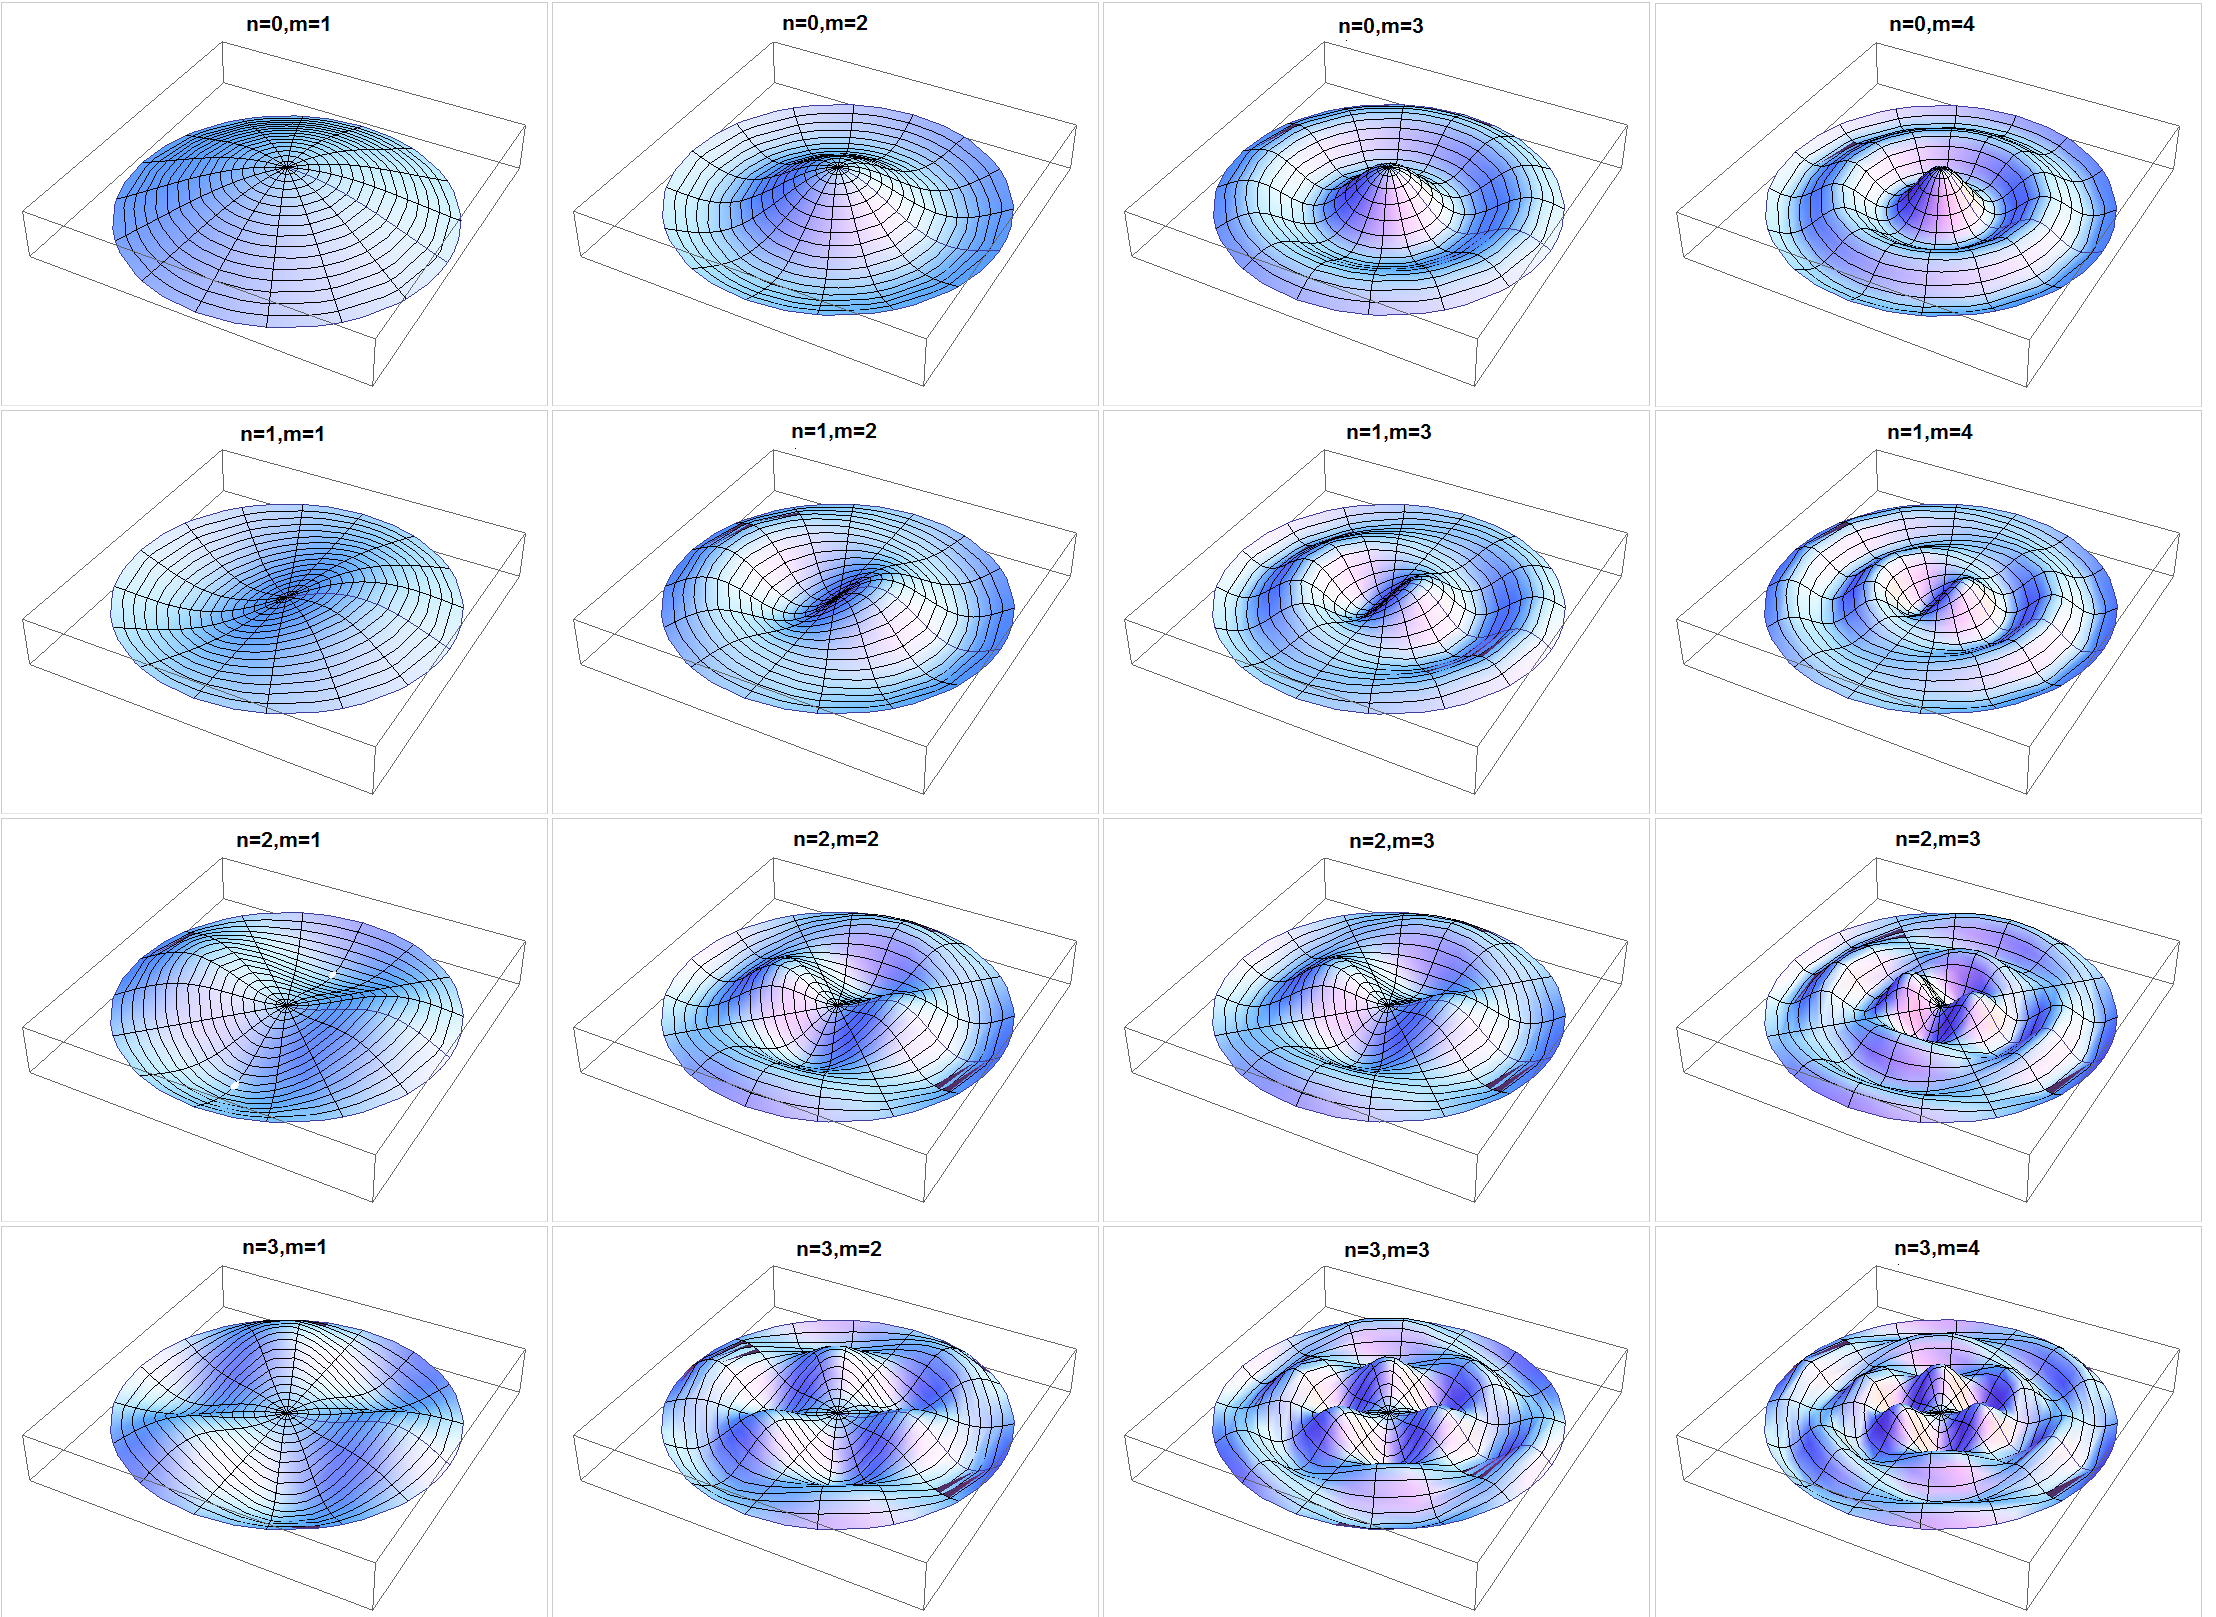
\includegraphics[width=1.1\textwidth]{DrumVibration1.png}}
		\caption{Solutions of the 2D wave equation on a disc (representing the modes of vibration of a drum). Note that this figure switches $m$ and $n$ from our usage. (source: \href{http://www.bio-physics.at/wiki/index.php?title=File:Vibrations.png}{bio-physics-wiki}).}
		\label{fig:wave2d}
	\end{figure}
\end{enumerate}

\subsubsection{More General Case}

So far, we have only considered a certain case of the wave equation - with wave speed $c=1$, the initial speed being zero everywhere, and radius 1 in the disc case. Out of interest, we now state the solutions in the general case:

\begin{enumerate}
	\item \textbf{General case on a rectangle.}
	
	We solve
	\[
	u_{tt} = c^2(u_{xx} + u_{yy}), \quad 0 \leq x \leq a, \,\, 0 \leq y \leq b
	\]
	with the following boundary and initial conditions
	\begin{equation*}
		\begin{alignedat}{2}
			u(0,y,t) &= u(a,y,t) = 0, \qquad u(x,y,0) &&= f(x,y), \\
			u(x,0,t) &= u(x,b,t) = 0, \qquad u_t(x,y,0) &&= g(x,y).
		\end{alignedat}
	\end{equation*}
	The general solution is
	\[
	u(x,y,t) = \sum_{n=1}^{\infty} \sum_{m=1}^{\infty} \left(A_{mn}\cos(\lambda_{mn}t) + A_{mn}^*\sin(\lambda_{mn}t) \right) \sin(\mu_m x) \sin(\nu_n y).
	\]
	where
	\[
	\mu_m = \frac{m\pi}{a}, \quad \nu_n = \frac{n\pi}{b}, \quad \lambda_{mn} = c\sqrt{\mu_m^2 + \nu_n^2},
	\]
	and the coefficients are given by
	\begin{align*}
		A_{mn} &= \frac{4}{ab} \int_0^a \int_0^b f(x,y) \sin(\mu_m x) \sin(\nu_n y) \,dy\,dx, \\
		A_{mn}^* &= \frac{4}{ab\lambda_{mn}} \int_0^a \int_0^b g(x,y) \sin(\mu_m x) \sin(\nu_n y) \,dy\,dx.
	\end{align*}
	
	\item \textbf{General case on a disc.}
	
	We solve
	\[
	\p_{tt}u = c^2\left(u_{rr} + \frac{1}{r}u_r + \frac{1}{r^2}u_{\theta\theta}\right), \quad 0 \leq r \leq a
	\]
	with the following boundary and conditions
	\begin{align*}
		u(r,\theta,0) &= f(r,\theta), \qquad u(a,\theta,t) = 0, \\
		u_t(r,\theta,0) &= g(r,\theta).
	\end{align*}
	The general solution is
	\begin{align*}
		u(r,\theta,t) = &\sum_{m=0}^{\infty} \sum_{n=1}^{\infty} \underbrace{\left(A_{mn}\cos(m\theta) + B_{mn}\sin(m\theta)\right) J_m(\lambda_{mn}r) \cos(c\lambda_{mn}t)}_{u_{mn}(r,\theta,t)} \\
		+ &\sum_{m=0}^{\infty} \sum_{n=1}^{\infty} \underbrace{\left(A_{mn}^*\cos(m\theta) + B_{mn}^*\sin(m\theta)\right) J_m(\lambda_{mn}r) \sin(c\lambda_{mn}t)}_{u_{mn}^*(r,\theta,t)},
	\end{align*}
	where
	\[
	\lambda_{mn} = \frac{\mu_{mn}}{a},
	\]
	and $\mu_{mn}$ is the $n$th positive zero of $J_m$. So we can see that the solution is split into two series - one relating to the initial shape, the other to the initial velocity.
	
	The coefficients related to $u_{mn}(r,\theta,t)$ are
	\begin{align}
		A_{0n} &= \frac{1}{\pi a^2J_1^2(\mu_{0n})} \int_0^{2\pi} \int_0^a f(r,\theta) J_0(\lambda_{0n}r) r \,dr\,d\theta \\
		\label{eq:wave2dgen1}
		A_{mn} &= \frac{2}{\pi a^2J_{m+1}^2(\mu_{mn})} \int_0^{2\pi} \int_0^a f(r,\theta) \cos(m\theta) J_m(\lambda_{mn}r) r \,dr\,d\theta \\
		B_{mn} &= \frac{2}{\pi a^2J_{m+1}^2(\mu_{mn})} \int_0^{2\pi} \int_0^a f(r,\theta) \sin(m\theta) J_m(\lambda_{mn}r) r \,dr\,d\theta,
	\end{align}
	and the coefficients related to $u_{mn}^*(r,\theta,t)$ are
	\begin{align}
		A_{0n}^* &= \frac{1}{\pi c\mu_{0n} aJ_1^2(\mu_{0n})} \int_0^{2\pi} \int_0^a g(r,\theta) J_m(\lambda_{0n}r) r \,dr\,d\theta \\
		A_{mn}^* &= \frac{2}{\pi c\mu_{mn} aJ_{m+1}^2(\mu_{mn})} \int_0^{2\pi} \int_0^a g(r,\theta) \cos(m\theta) J_m(\lambda_{mn}r) r \,dr\,d\theta \\
		B_{mn}^* &= \frac{2}{\pi c\mu_{mn} aJ_{m+1}^2(\mu_{mn})} \int_0^{2\pi} \int_0^a g(r,\theta) \sin(m\theta) J_m(\lambda_{mn}r) r \,dr\,d\theta,
	\end{align}
	for $m,n \in \mathbb{N}$.
\end{enumerate}

\subsubsection{Examples}

Note that while these examples follow the statement of the general case of the 2D wave equation, they are in fact (nearly) example of the specific cases we solved in \Cref{sec:waveeqn2dne}. The only difference is that in \Cref{eg:waveeqn2drect}, we take $c=6$ instead of $c=1$ for wave speed.

\begin{eg}\label{eg:waveeqn2drect}
	A $2 \times 3$ rectangular membrane, with $c=6$, is deformed to have an initial shape given by
	\[
	f(x,y) = xy(2-x)(3-y).
	\]
	The edges of this membrane are kept fixed, and it is released at $t=0$. We wish to find an expression for the shape of the membrane for $t>0$.
	
	Since the membrane starts from rest, $A_{mn}^* = 0$ immediately, Then
	\begin{align*}
		A_{mn} &= \frac{4}{ab} \int_0^a \int_0^b f(x,y) \sin(\mu_m x) \sin(\nu_n y) \,dy\,dx \\
		&= \frac23 \int_0^2 \int_0^3 xy(2-x)(3-y) \sin\left(\frac{m\pi x}{2}\right) \sin\left(\frac{n\pi y}{3}\right) \,dy\,dx \\
		&= \frac23 \int_0^2 x(2-x) \sin\left(\frac{m\pi x}{2}\right) \,dx \int_0^3 y(3-y) \sin\left(\frac{n\pi y}{3}\right) \,dy \\
		&= \frac23 \left(\frac{16\left(1+(-1)^{m+1}\right)}{\pi^3 m^3}\right) \left(\frac{54\left(1+(-1)^{n+1}\right)}{\pi^3 n^3}\right) \\
		&= \frac{576}{\pi^6} \frac{\left(1+(-1)^{m+1}\right) \left(1+(-1)^{n+1}\right)}{m^3n^3}.
	\end{align*}
	In this working, we write
	\[
	\int_0^2 x(2-x) \sin\left(\frac{m\pi x}{2}\right) \,dx = 2\int_0^2 x \sin\left(\frac{m\pi x}{2}\right) \,dx - \int_0^2 x^2 \sin\left(\frac{m\pi x}{2}\right) \,dx,
	\]
	then use the fact that
	\begin{align*}
		\int x\sin(ax)\,dx &= -\frac{x\cos(ax)}{a} + \frac{\sin(ax)}{a^2} + C \\
		\int x^2\sin(ax)\,dx &= -\frac{x^2\cos(ax)}{a} + \frac{2x\sin(ax)}{a^2} + \frac{2\cos(ax)}{a^3} + C
	\end{align*}
	to find the definite integral between 0 and 2 for $a = \frac{m\pi}{2}$. A similar method works for calculating the second integral.
	
	The coefficients $\lambda_{mn}$ are given by
	\[
	\lambda_{mn} = 6\sqrt{\frac{m^2\pi^2}{2^2} + \frac{n^2\pi^2}{3^2}} = \pi\sqrt{9m^2+4n^2}.
	\]
	Assembling these pieces yields a general solution of
	\[
	u(x,y,t) = \frac{576}{\pi^6} \sum_{n=1}^{\infty} \sum_{m=1}^{\infty} \frac{\left(1+(-1)^{m+1}\right) \left(1+(-1)^{n+1}\right)}{m^3n^3} \cos\left(\pi\sqrt{9m^2+4n^2}t\right) \sin\left(\frac{m\pi x}{2}\right) \sin\left(\frac{n\pi y}{3}\right).
	\]
\end{eg}

\begin{exercise}
	Suppose you are a masochist (why else would you attempt this?) In addition, suppose that in the previous example we also impose an initial velocity of $g(x,y) = \sin(2\pi x)$. Find the shape of the membrane for time $t>0$ in this case.
\end{exercise}

\begin{remark}
	With the 2D wave equation on a disc, if $f$ is such that $f(r,\theta)=f(r)$) (i.e. $f$ is radially symmetric), then for $m \neq 0$, $A_{mn} = 0$ and $B_{mn} = 0$ also. In other words, there are only the $A_{0n}$ terms.
	
	Likewise, if $g$ is radially symmetric, then there are only $A_{0n}^*$ terms.
\end{remark}

\begin{proof}
	Beginning with \Cref{eq:wave2dgen1},
	\begin{align*}
		A_{mn} &= \frac{2}{\pi a^2J_{m+1}^2(\mu_{mn})} \int_0^{2\pi} \int_0^a f(r,\theta) \cos(m\theta) J_m(\lambda_{mn}r) r \,dr\,d\theta,
		\intertext{and replacing $f(r,\theta)$ with $f(r)$,}
		&= (\cdots) \int_0^{2\pi} \int_0^a f(r) \cos(m\theta) J_m(\lambda_{mn}r) r \,dr\,d\theta \\
		&= (\cdots)  \int_0^a f(r) J_m(\lambda_{mn}r) r \,dr \underbrace{\int_0^{2\pi} \cos(m\theta) \,d\theta}_{=0},
	\end{align*}
	and similarly for $B_{mn}$.
\end{proof}

This remark is very useful in the following example:

\begin{eg}
	Solve the wave equation in two dimensions with $a=c=1$ and initial conditions
	\[
	f(r,\theta)=1-r^4, \quad g(r,\theta)=0.
	\]
	Because $g(r,\theta)=0$, we do not need to worry about the $A_{mn}^*$ and $B_{mn}^*$ terms. In addition, because $f$ is radially symmetric, we only need to compute $A_{0n}$:
	\begin{align*}
		A_{0n} &= \frac{1}{\pi J_1^2(\mu_{0n})} \int_0^{2\pi} \int_0^1 f(r) J_0(\mu_{0n}r) r \,dr\,d\theta \\
		&= \frac{1}{\pi J_1^2(\mu_{0n})} \int_0^{2\pi} \,d\theta \int_0^1 f(r) J_m(\mu_{0n}r) r \,dr \\
		&= \frac{2}{J_1^2(\mu_{0n})} \int_0^1 (1-r^4) J_0(\mu_{0n}r) r \,dr.
	\end{align*}
	We make the substitution $x = \mu_{0n}r$:
	\begin{align*}
		&= \frac{2}{\mu_{0n}^2 J_1^2(\mu_{0n})} \int_0^{\mu_{0n}} \left( 1-\frac{x^4}{\mu_{0n}^4} \right) J_0(x) x \,dx \\
		&= \frac{2}{\mu_{0n}^2 J_1^2(\mu_{0n})} \left( \underbrace{\int_0^{\mu_{0n}} xJ_0(x) \,dx}_{A} - \frac{1}{\mu_{0n}^4} \underbrace{\int_0^{\mu_{0n}} x^5J_0(x) \,dx}_{B}\right). 
	\end{align*}
	From here, we find\footnote{The first of these can be found by integrating the power series for $J_0(x)$ in \Cref{eq:besselfirstkind}, making use of the fact that $\Gamma(k+1)=k!$:
		\[
		xJ_0(x) = x \sum_{k=0}^{\infty} (-1)^k\frac{(\frac{x^2}{4})^k}{k!\Gamma(k+1)} = x \sum_{k=0}^{\infty} \frac{(-1)^k}{4^k(k!)^2}x^{2k+1}.
		\]
		Therefore
		\begin{align*}
			\int xJ_0(x) \,dx &= \int \sum_{k=0}^{\infty} \frac{(-1)^k}{4^k(k!)^2}x^{2k+1} \,dx = \sum_{k=0}^{\infty} \frac{(-1)^k}{4^k(k!)^2(2k+2)}x^{2k+2} \\
			&= \frac{x^2}{2} \sum_{k=0}^{\infty} \frac{(-1)^k}{4^kk!(k+1)!}x^{2k} = x \cdot \frac{x}{2} \sum_{k=0}^{\infty} (-1)^k\frac{(\frac{x^2}{4})^k}{k!\Gamma(k+2)} = xJ_1(x).
		\end{align*}
		Alternatively, we know from \cite[Eq. 9.1.30]{olver} that
		\[
		\frac{d}{dx}\left(x^pJ_p(x)\right) = x^pJ_{p-1}(x),
		\]
		and setting $p=1$ and integrating both sides gives the desired result.}
	\begin{align*}
		A = \int_0^{\mu_{0n}} xJ_0(x) \,dx &= \left[xJ_1(x)\right]_0^{\mu_{0n}} = \mu_{0n}J_1(\mu_{0n}) \\
		B = \int_0^{\mu_{0n}} x^5J_0(x) \,dx &= \left[x^5J_1(x) - 4x^4J_2(x) + 8x^3J_3(x)\right]_0^{\mu_{0n}} \\
		&= \mu_{0n}^5J_1(\mu_{0n}) - 4\mu_{0n}^4J_2(\mu_{0n}) + 8\mu_{0n}^3J_3(\mu_{0n}).
	\end{align*}
	It follows that
	\[
	A_{0n} = \frac{2}{\mu_{0n}^2 J_1^2(\mu_{0n})} \left(A - \frac{1}{\mu_{0n}^4}B\right) = \frac{8\left(\mu_{0n}J_2(\mu_{0n}) - 2J_3(\mu_{0n})\right)}{\mu_{0n}^3J_1^2(\mu_{0n})},
	\]
	so that finally
	\[
	u(r,\theta,t) = \sum_{n=1}^{\infty} \frac{8\left(\mu_{0n}J_2(\mu_{0n}) - 2J_3(\mu_{0n})\right)}{\mu_{0n}^3J_1^2(\mu_{0n})} J_0(\mu_{0n}r)\cos(\mu_{0n}t).
	\]
\end{eg}